\documentclass[conference]{IEEEtran}
\usepackage[utf8]{inputenc}
\usepackage[T1]{fontenc}
\usepackage{amsmath}
\usepackage{booktabs}
\usepackage{cite}
\usepackage{graphicx}
\usepackage{placeins}
\usepackage{url}

\title{Predicting Answer Correctness from Token-Level Top-10 Probability Curves}

\author{
\IEEEauthorblockN{Özgür Aslan}
\IEEEauthorblockA{Yildiz Technical University\\
Computational Semantics Final Project Report}
}

\begin{document}
\maketitle

\begin{abstract}
This report studies whether a language model's token-level uncertainty can
predict the correctness of its mathematical answers. For each Turkish GSM8K
question, Qwen3-4B was sampled ten times and the sum of the probabilities of
the ten most likely next tokens was recorded at every generated position. The
resulting curve is close to one for most tokens, but small drops indicate that
probability mass is spreading beyond the top candidates. Only mixed questions,
where the same prompt produced both correct and incorrect answers, were kept so
that the classifier must distinguish answer quality rather than question
difficulty. The final dataset contains 1,320 answers from 132 mixed questions.
Curve statistics, dip features, answer length, and within-question relative
features were used with several tree-based classifiers. The best ROC-AUC was
0.6151 with Gradient Boosting, while Random Forest reached the best accuracy of
0.5781 against a 0.5250 majority baseline. The results show that the top-10
probability curve carries a real but weak correctness signal.
\end{abstract}

\section{Introduction}
Reasoning models often produce several plausible solution paths for the same
mathematical problem. In a reinforcement-learning setting such as GRPO, it is
useful to understand whether incorrect answers leave a detectable trace before
the final answer is emitted. This project tests a simple hypothesis: when the
model is about to choose a wrong reasoning branch, its next-token distribution
becomes less concentrated, and this hesitation appears as a drop in the summed
probability of the top-10 tokens.

The task is intentionally harder than ordinary answer classification. The input
to the classifier is not the generated text, the question, or the final numeric
answer. It only receives the graph-derived signal extracted during generation.
Furthermore, the dataset keeps only questions for which the same model produced
both correct and incorrect samples. This prevents a classifier from simply
learning that some questions are easy while others are hard.

The project repository is available at
\url{https://github.com/ozguraslank/ytu-nlp-project}.

\section{Data Generation}
The source questions are Turkish grade-school math problems from local CSV
samples derived from \texttt{ytu-ce-cosmos/gsm8k\_tr}, a Turkish GSM8K dataset
hosted on Hugging Face~\cite{huggingfacegsm8ktr} and based on
GSM8K~\cite{cobbe2021gsm8k}. The experiment did not run over the full Turkish
GSM8K dataset. Instead, the generation script loads 250 training and 250 test
questions, prompts \texttt{unsloth/Qwen3-4B} with a Turkish math assistant
instruction, disables Qwen's explicit thinking blocks, and samples ten answers
per question using vLLM. Sampling used temperature 0.7, top-p 0.8, a maximum of
1024 generated tokens, and top-10 log-probability output for every generated
token.

For token position $t$, vLLM returns log-probabilities for the highest scoring
tokens. The signal used in this project is
\begin{equation}
    s_t = \sum_{k=1}^{10} \exp(\ell_{t,k}),
\end{equation}
where $\ell_{t,k}$ is the $k$th largest log-probability at position $t$. In a
highly concentrated distribution, $s_t$ is close to one. Lower values mean that
more probability mass has moved outside the ten most likely tokens.

Each answer was labeled by parsing the numeric result after the required
\texttt{\#\#\#\#} marker, with a fallback to the last number in the answer text.
Turkish decimal and thousands separators were normalized before comparison with
the gold answer. A question was kept only if at least one of its ten samples was
correct and at least one was incorrect.

\begin{table}[t]
\caption{Final dataset after filtering to mixed questions.}
\label{tab:data}
\centering
\begin{tabular}{lrrrr}
\toprule
Split & Questions & Answers & Correct & Incorrect \\
\midrule
Train & 68 & 680 & 376 & 304 \\
Test & 64 & 640 & 336 & 304 \\
\midrule
Total & 132 & 1320 & 712 & 608 \\
\bottomrule
\end{tabular}
\end{table}

Table~\ref{tab:data} summarizes the final data. Among the 500 sampled prompts
(250 train and 250 test), only 132 questions produced mixed answer sets
containing both labels. The split is still by question, so sibling answers of
the same question never appear in both training and test data.

\section{Top-10 Probability Curves}
Figure~\ref{fig:single} shows one mixed question with five correct and five
incorrect answers. The y-axis is deliberately zoomed because the raw top-10
probability mass is saturated near one. On a full 0--1 axis, almost all curves
would appear flat. In this example, several incorrect answers show deeper and
longer drops than most correct answers, especially in the middle and later parts
of the generation.

\begin{figure}[t]
\centering
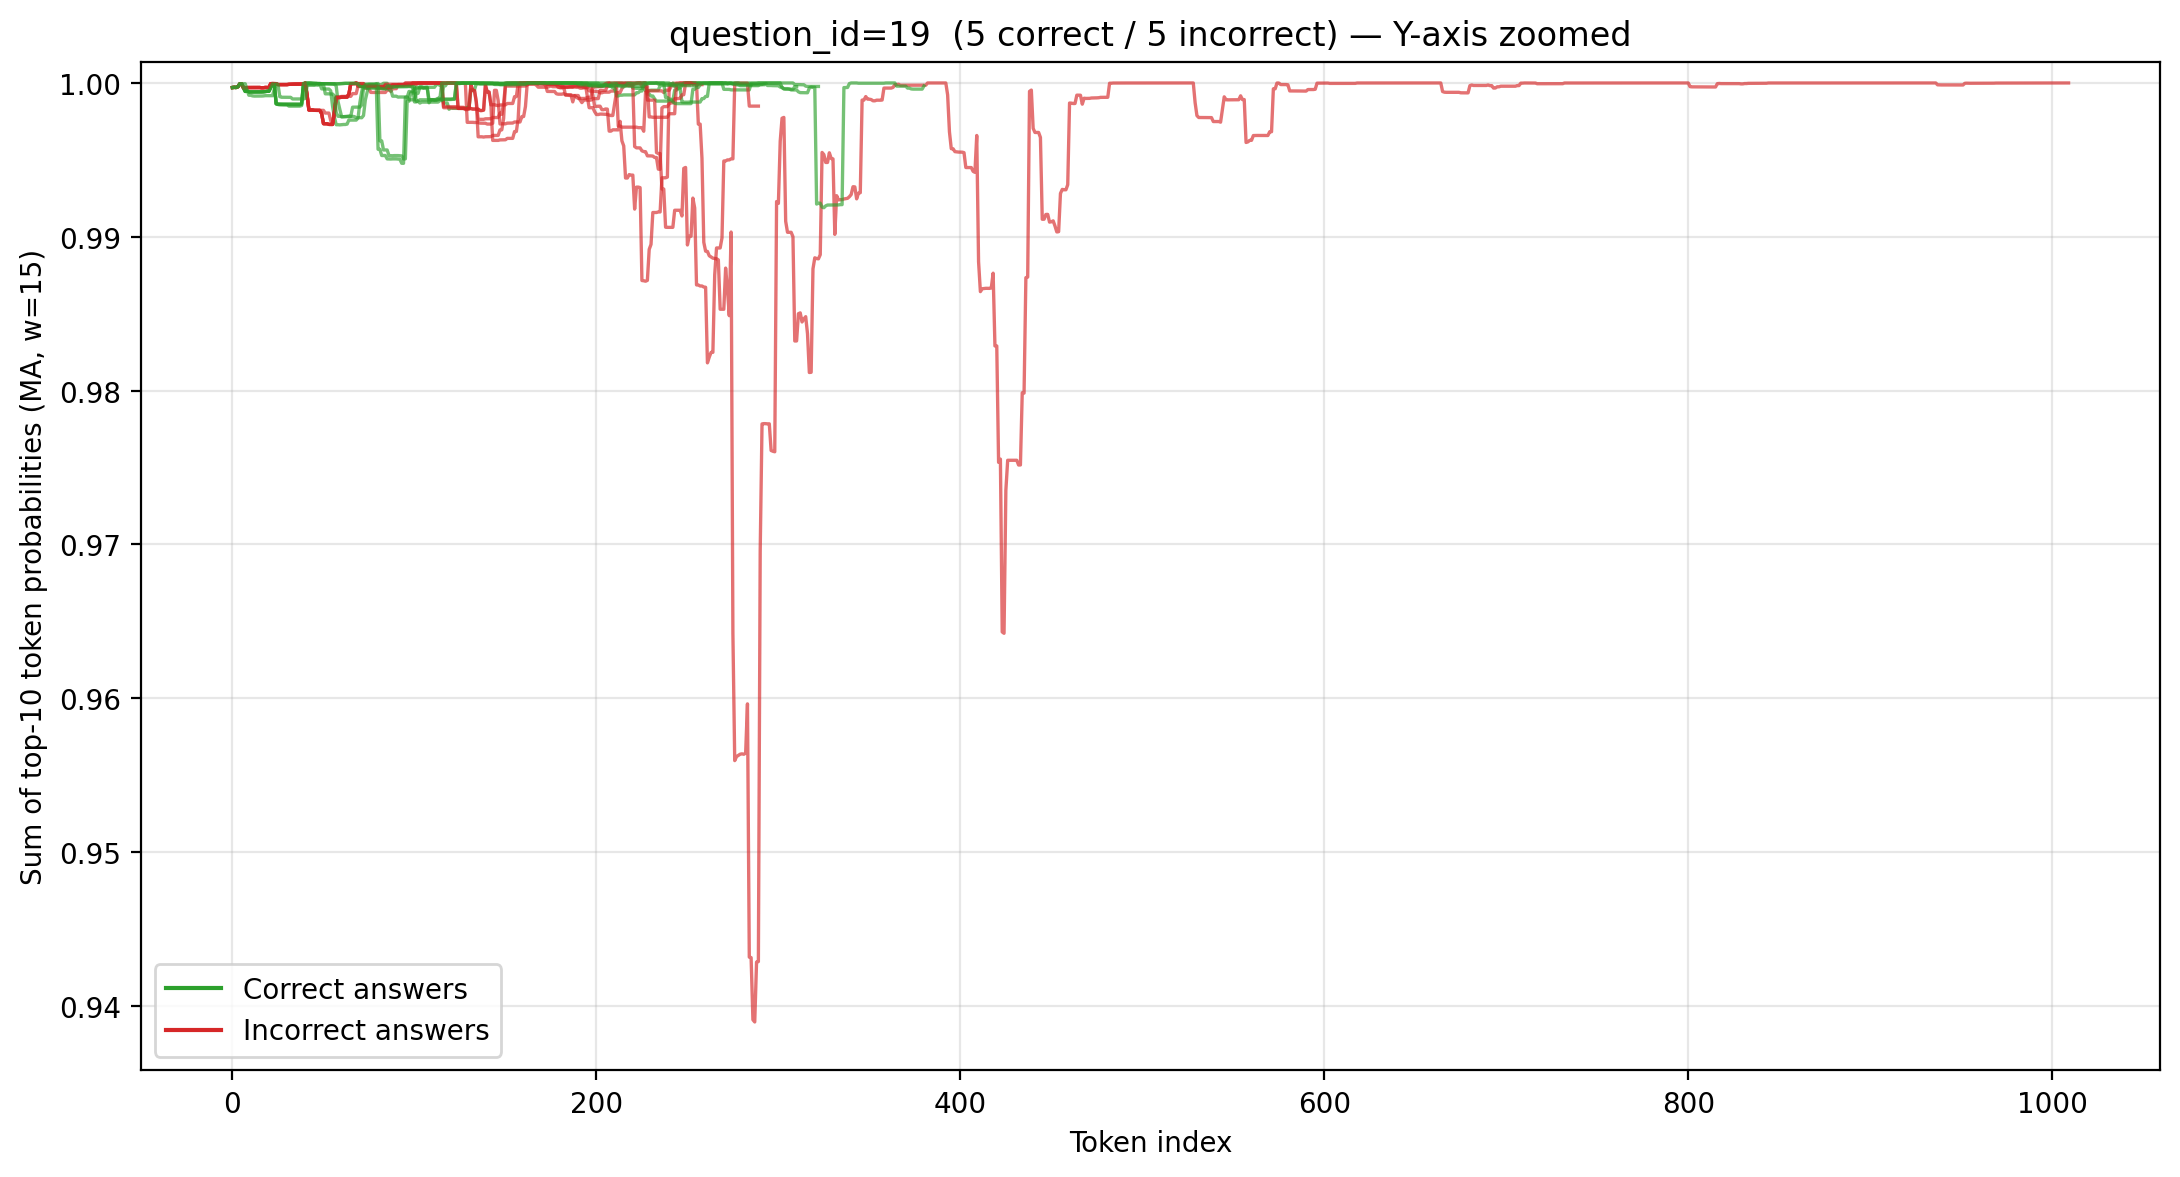
\includegraphics[width=\linewidth]{img/top10_ma_q19.png}
\caption{Moving-average top-10 probability curves for one mixed question.
Green curves are correct answers and red curves are incorrect answers. The
y-axis is zoomed to expose small deviations near one.}
\label{fig:single}
\end{figure}

A single question is only anecdotal, so the grid in Fig.~\ref{fig:grid}
compares several mixed questions. The pattern is heterogeneous: some questions
show clear uncertainty dips in incorrect answers, while others show overlap or
even dips in correct answers. This visual overlap already suggests that the
classification task should be possible but limited.

\begin{figure*}[t]
\centering
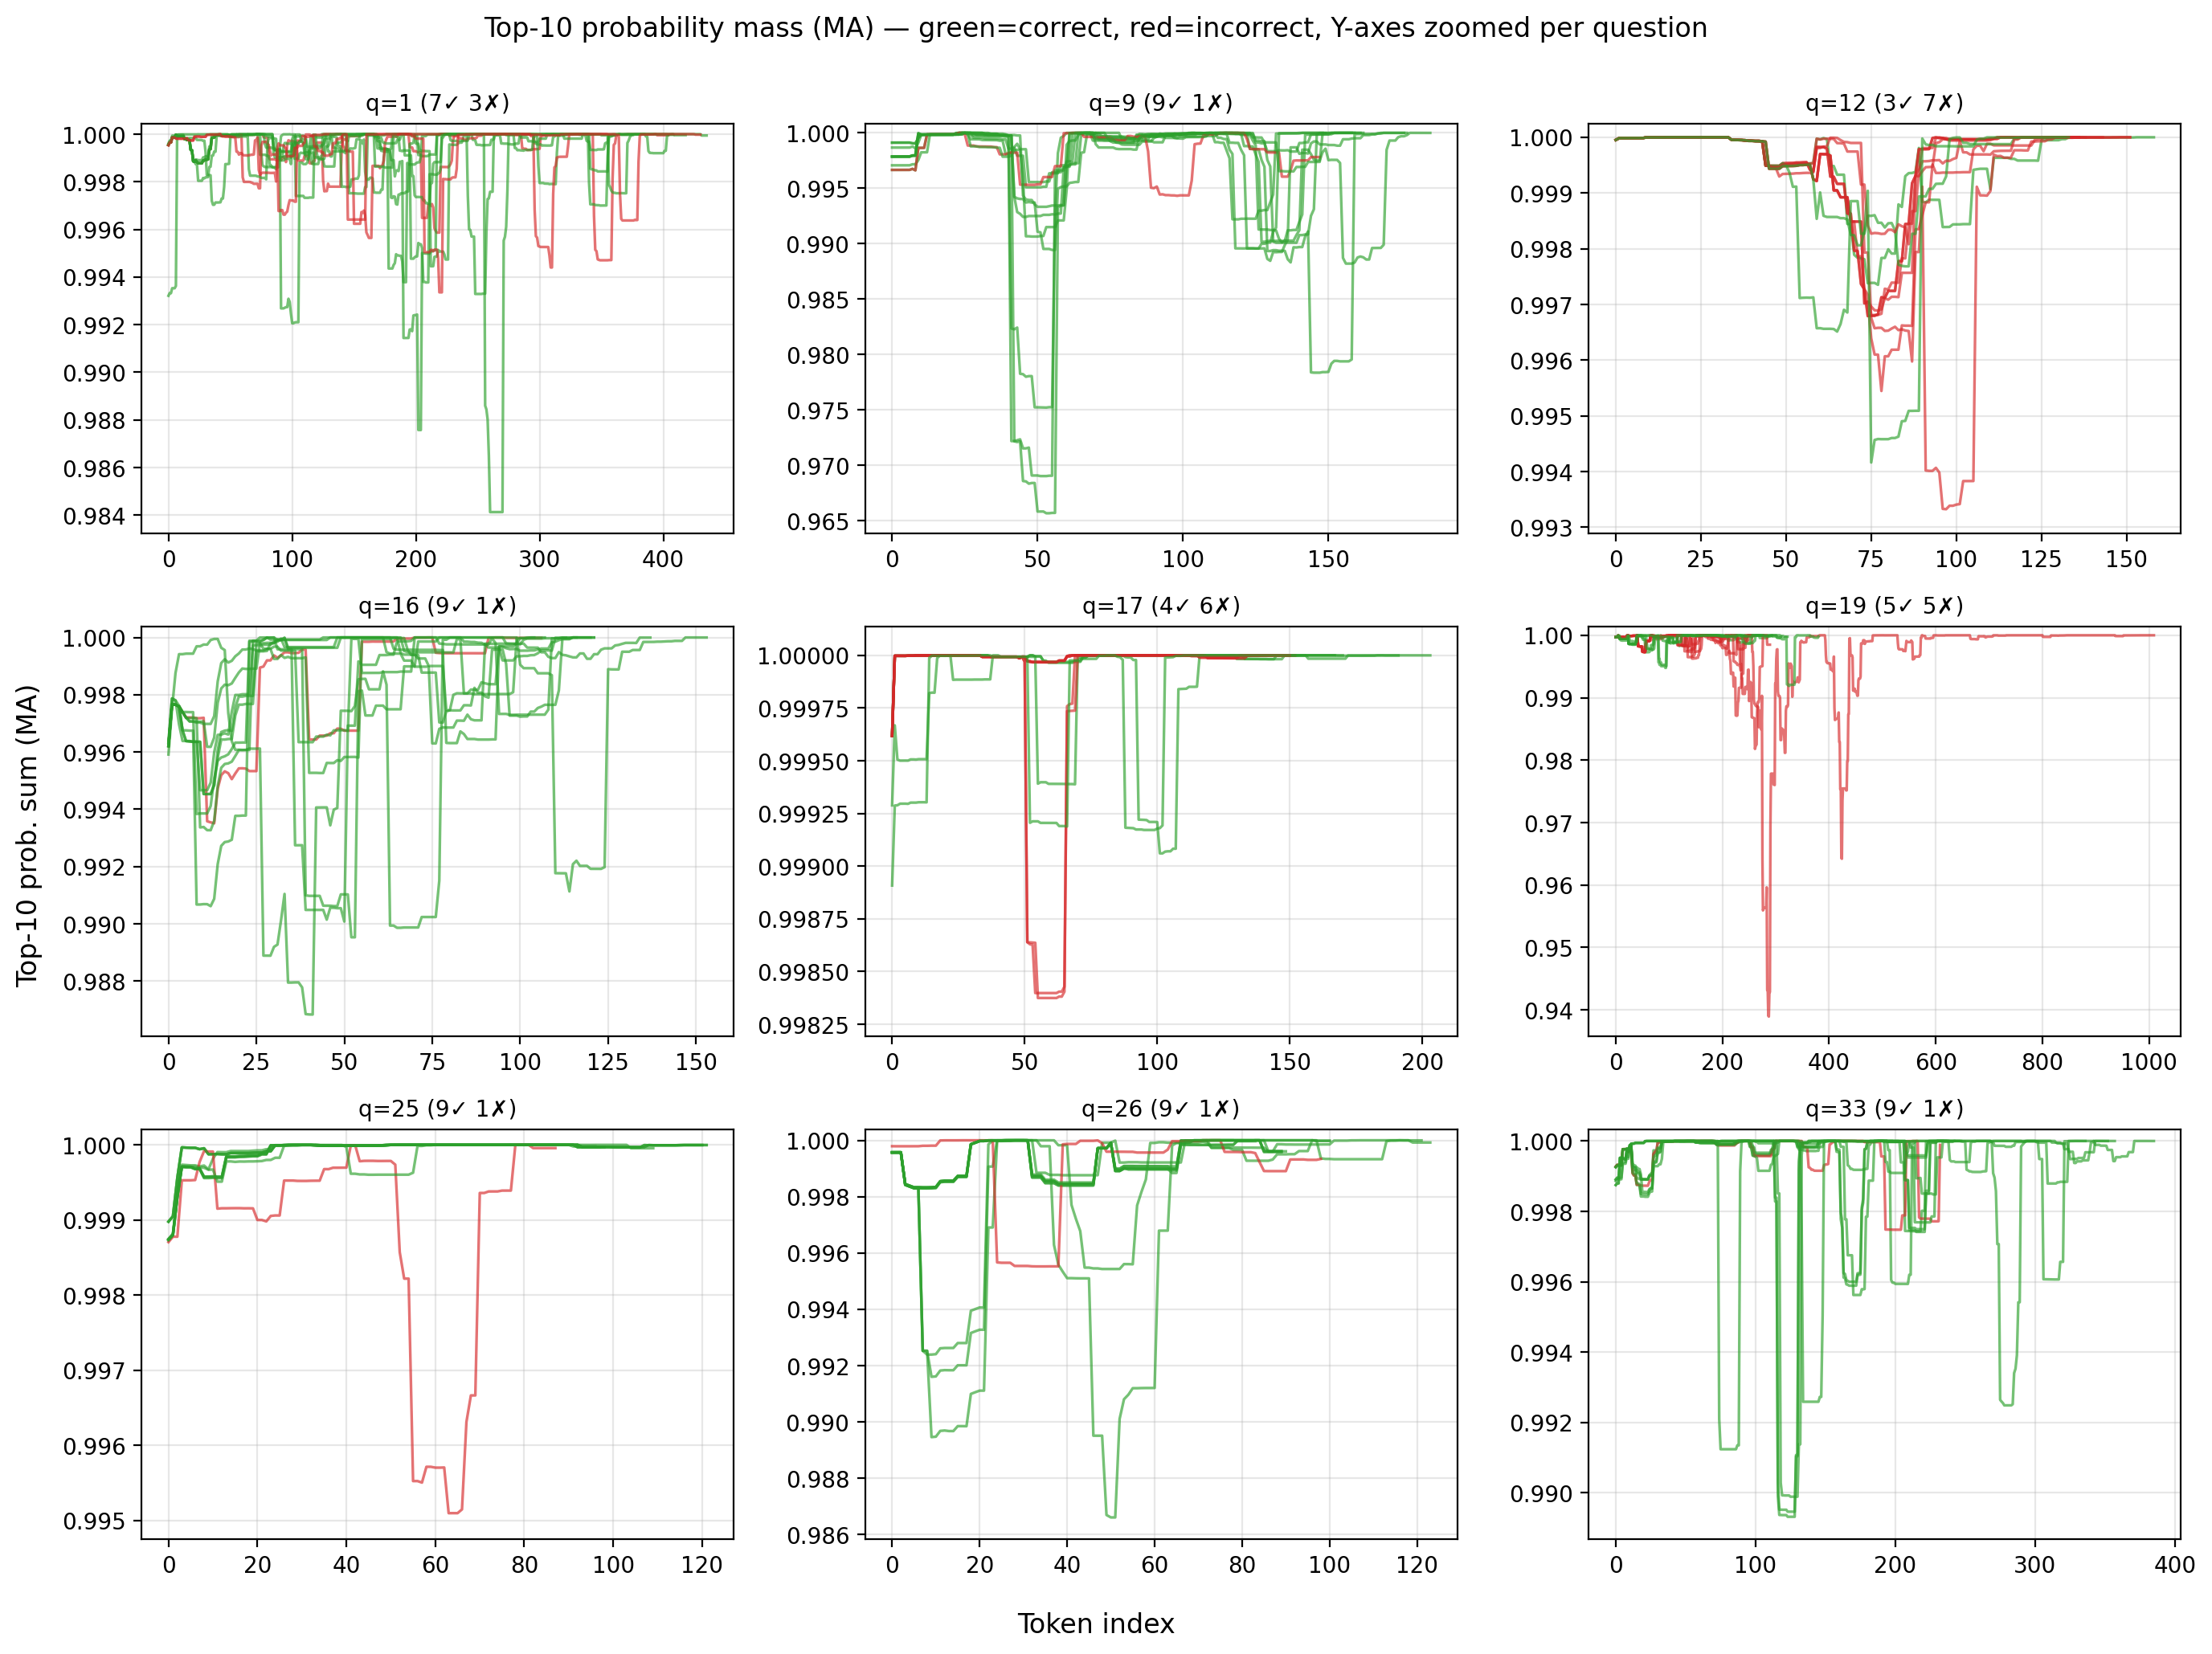
\includegraphics[width=0.92\textwidth]{img/top10_ma_grid.png}
\caption{Small-multiple view of nine mixed questions. Each panel has an
independently zoomed y-axis. The signal is not perfectly aligned across
questions, which motivates within-question relative features.}
\label{fig:grid}
\end{figure*}

The visual separation depends on the label balance inside the ten generated
answers for a question. When roughly four or five of the ten answers are wrong,
the red and green curves are usually easier to distinguish, and the red curves
more often sit lower or contain deeper dips. When only one or two answers are
wrong, the distinction is much less stable: a correct answer can have a
red-like dip, or the few incorrect answers may not go below the green curves.
Thus, the clearest qualitative evidence appears in nearly balanced mixed
questions rather than in questions with only a small minority of wrong answers.

\section{Feature Extraction and Models}
For every answer, features were computed from the same window-15 moving-average
curve used in the plots. The raw features include mean, standard deviation,
minimum, maximum, median, percentiles, linear slope, first/middle/last-third
means, last-minus-first difference, location of the minimum, sharpest local
drop, roughness, fractions below 0.90, 0.95, and 0.99, total uncertainty area
$\sum_t (1-s_t)$, answer length, and log length.

Absolute confidence differs strongly from one question to another. Therefore,
each raw feature was also transformed within its group of ten sibling answers.
For a feature value $x_{iq}$ for answer $i$ of question $q$, the relative
z-score is
\begin{equation}
    z_{iq} = \frac{x_{iq} - \mu_q}{\sigma_q + 10^{-9}}.
\end{equation}
A within-question rank feature was also added. The final representation is the
concatenation of raw, within-question z-scored, and within-question ranked
features.

Five classifiers were evaluated: XGBoost, CatBoost, Gradient Boosting, Random
Forest, and LightGBM. All models were trained on the 68 training questions and
tested on the 64 held-out questions. Accuracy, F1 score for the correct class,
and ROC-AUC were reported. The majority-class baseline on the test set is
0.5250 because 336 of 640 test answers are correct.

\section{Results}
Table~\ref{tab:results} gives the Step 3 modeling results. All models improve
over the majority baseline, but the margin is modest. Random Forest obtains the
highest accuracy, 0.5781, while Gradient Boosting obtains the highest ROC-AUC,
0.6151. ROC-AUC is especially important here because the task is a confidence
ranking problem: it asks whether the graph signal tends to assign higher
correctness probability to correct answers even when the default 0.5 threshold
is imperfect.

\begin{table}[t]
\caption{Classification results on 640 held-out answers.}
\label{tab:results}
\centering
\begin{tabular}{lccc}
\toprule
Model & Accuracy & F1 & ROC-AUC \\
\midrule
Majority baseline & 0.5250 & -- & -- \\
XGBoost & 0.5578 & 0.5928 & 0.5623 \\
CatBoost & 0.5750 & 0.6233 & 0.6093 \\
Gradient Boosting & 0.5734 & 0.6106 & \textbf{0.6151} \\
Random Forest & \textbf{0.5781} & 0.6143 & 0.6073 \\
LightGBM & 0.5578 & 0.6053 & 0.5875 \\
\bottomrule
\end{tabular}
\end{table}

The class-level reports show the same trade-off. CatBoost has the highest
correct-answer recall, 0.670, but only 0.470 recall for incorrect answers.
Random Forest is more balanced, with 0.510 recall for incorrect answers and
0.640 recall for correct answers. Thus, the graph features are better at
identifying likely-correct answers than reliably catching every incorrect one.

\section{Discussion}
The results support the main hypothesis, but only weakly. The clearest visual
separation appears when a question has several correct and several incorrect
answers, because the red curves can be compared against multiple green sibling
curves. With only one or two incorrect answers, individual variation dominates:
some correct answers contain deep dips because the model explores a difficult
but ultimately valid reasoning step, while some incorrect answers remain highly
confident until the final numeric mistake. This explains why the best AUC is in
the low 0.60 range rather than close to perfect separation.

The top-10 probability sum is also a limited uncertainty measure. Because the
model often assigns almost all probability mass to the top ten tokens, the
signal is compressed near one. The generated arrays occasionally exceed one by a
tiny amount due to floating-point and log-probability reconstruction effects,
which is harmless for relative curve features but reinforces that the useful
variation is very small. A sharper signal would likely include the sampled
token's own probability, full entropy over more of the vocabulary, or
token-level likelihood of the complete answer.

Another limitation is dataset size and scope. The experiment did not perform
prediction over the whole Turkish GSM8K dataset; it used local samples of 250
training and 250 test questions. Only 132 of these 500 sampled questions were
mixed, so the held-out set is meaningful but still small, especially because all
evaluation is by question. Hyperparameter tuning and additional mixed questions
would be the next steps before making stronger claims.

\section{Conclusion}
This project tested whether answer correctness can be predicted from the shape
of a top-10 token probability curve. On 1,320 generated answers from 132 mixed
Turkish GSM8K questions, balanced mixed questions often showed clearer
separation between correct and incorrect curves, while questions with only one
or two wrong answers were more ambiguous. Machine-learning models trained on
curve features improved over a 0.5250 majority baseline, with the best accuracy
reaching 0.5781 and the best ROC-AUC reaching 0.6151. The signal is therefore
real but weak: top-10 probability curves reveal some model hesitation, but they
are not sufficient alone for highly reliable correctness prediction.

\FloatBarrier

\begin{thebibliography}{99}

\bibitem{cobbe2021gsm8k}
K.~Cobbe, V.~Kosaraju, M.~Bavarian, M.~Chen, H.~Jun, L.~Kaiser, M.~Plappert,
J.~Tworek, J.~Hilton, R.~Nakano, C.~Hesse, and J.~Schulman, ``Training
verifiers to solve math word problems,'' \emph{arXiv preprint
arXiv:2110.14168}, 2021.

\bibitem{huggingfacegsm8ktr}
Yildiz Technical University Computer Engineering Department Cosmos Research
Group, ``\texttt{ytu-ce-cosmos/gsm8k\_tr},'' Hugging Face dataset. [Online].
Available: \url{https://huggingface.co/datasets/ytu-ce-cosmos/gsm8k_tr}.
Accessed: Jun. 15, 2026.

\bibitem{qwen2025qwen3}
Qwen Team, ``Qwen3 technical report,'' \emph{arXiv preprint arXiv:2505.09388},
2025.

\bibitem{kwon2023vllm}
W.~Kwon, Z.~Li, S.~Zhuang, Y.~Sheng, L.~Zheng, C.~Yu, J.~Gonzalez,
H.~Zhang, and I.~Stoica, ``Efficient memory management for large language model
serving with PagedAttention,'' in \emph{Proc. ACM SIGOPS Symp. Operating
Systems Principles}, 2023.

\bibitem{chen2016xgboost}
T.~Chen and C.~Guestrin, ``XGBoost: A scalable tree boosting system,'' in
\emph{Proc. ACM SIGKDD Int. Conf. Knowledge Discovery and Data Mining}, 2016,
pp.~785--794.

\bibitem{dorogush2018catboost}
A.~V. Dorogush, V.~Ershov, and A.~Gulin, ``CatBoost: gradient boosting with
categorical features support,'' \emph{arXiv preprint arXiv:1810.11363}, 2018.

\bibitem{ke2017lightgbm}
G.~Ke, Q.~Meng, T.~Finley, T.~Wang, W.~Chen, W.~Ma, Q.~Ye, and T.-Y. Liu,
``LightGBM: A highly efficient gradient boosting decision tree,'' in
\emph{Advances in Neural Information Processing Systems}, 2017.

\bibitem{pedregosa2011sklearn}
F.~Pedregosa \emph{et al.}, ``Scikit-learn: Machine learning in Python,''
\emph{Journal of Machine Learning Research}, vol.~12, pp.~2825--2830, 2011.

\end{thebibliography}

\end{document}
